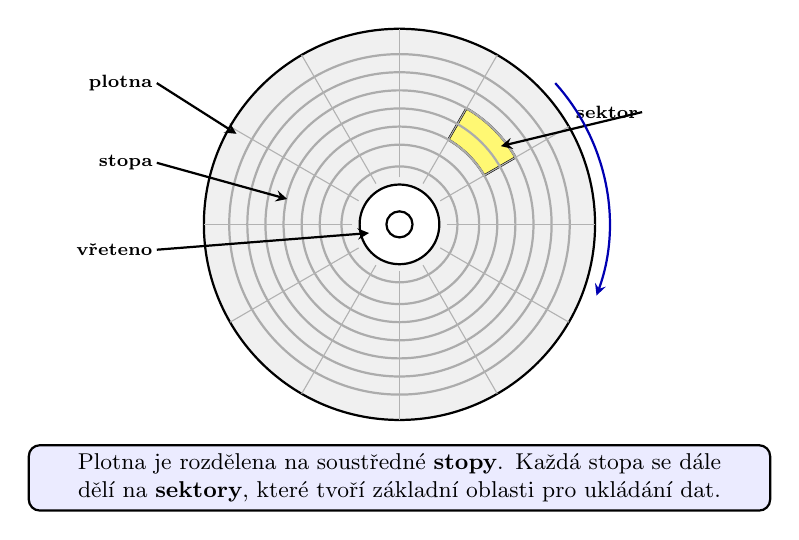
\begin{tikzpicture}[
scale=0.92,
transform shape,
x=1cm, y=1cm,
>=stealth,
every node/.style={font=\small},
platter/.style={draw, thick, fill=gray!12},
track/.style={draw, thick, gray!65},
sectorline/.style={draw, thin, gray!60},
highlight/.style={draw, thick, fill=yellow!55},
hub/.style={draw, thick, fill=white},
callout/.style={->, thick},
labelbox/.style={font=\scriptsize, fill=white, inner sep=1.5pt},
detailbox/.style={
    draw,
    thick,
    rounded corners,
    fill=yellow!12,
    align=center
},
bitcell/.style={
    draw,
    minimum width=0.42cm,
    minimum height=0.32cm,
    fill=white,
    font=\scriptsize
}
]

% =====================================================
% Plotna
% =====================================================

% Outer platter
\draw[platter] (0,0) circle (2.7);

% Highlighted sector on one track
\path[highlight]
(30:1.35)
arc (30:60:1.35)
-- (60:1.85)
arc (60:30:1.85)
-- cycle;

% Tracks
\foreach \r in {0.8,1.1,1.35,1.6,1.85,2.1,2.35}{
\draw[track] (0,0) circle (\r);
}

% Sector lines
\foreach \a in {0,30,60,90,120,150,180,210,240,270,300,330}{
\draw[sectorline] (\a:0.65) -- (\a:2.7);
}

% Hub / spindle
\draw[hub] (0,0) circle (0.55);
\draw[hub] (0,0) circle (0.18);
\node[font=\scriptsize] at (0,-0.02) {};

% Labels around platter
\node[labelbox, anchor=east] (labplatter) at (-3.35,1.95) {\textbf{plotna}};
\draw[callout] (labplatter.east) -- (-2.25,1.25);

\node[labelbox, anchor=east] (labtrack) at (-3.35,0.85) {\textbf{stopa}};
\draw[callout] (labtrack.east) -- (-1.55,0.35);

\node[labelbox, anchor=east] (labhub) at (-3.35,-0.35) {\textbf{vřeteno}};
\draw[callout] (labhub.east) -- (-0.42,-0.12);

\node[labelbox, anchor=east] (labsector) at (3.35,1.55) {\textbf{sektor}};
\draw[callout] (labsector.east) -- (1.40,1.08);

% Rotation arrow
\draw[->, thick, blue!70!black]
(2.15,1.95)
arc (42:-20:2.9);

% Bottom note
\node[
draw,
thick,
rounded corners,
fill=blue!8,
align=center,
font=\small,
text width=10.0cm
] at (0,-3.50) {
Plotna je rozdělena na soustředné \textbf{stopy}. Každá stopa se dále dělí na \textbf{sektory}, které tvoří základní oblasti pro ukládání dat.
};

\end{tikzpicture}
